\documentclass[12pt]{article}
\usepackage[utf8]{inputenc}

\usepackage{graphicx}
\graphicspath{ {./} }

\usepackage{listings}
\usepackage{color}

\definecolor{codegreen}{rgb}{0,0.6,0}
\definecolor{codegray}{rgb}{0.5,0.5,0.5}
\definecolor{codepurple}{rgb}{0.58,0,0.82}
\definecolor{backcolour}{rgb}{0.95,0.95,0.92}
 
\lstdefinestyle{mystyle}{
    backgroundcolor=\color{backcolour},   
    commentstyle=\color{codegreen},
    keywordstyle=\color{magenta},
    numberstyle=\tiny\color{codegray},
    stringstyle=\color{codepurple},
    basicstyle=\footnotesize,
    breakatwhitespace=false,         
    breaklines=true,                 
    captionpos=b,                    
    keepspaces=true,                 
    numbers=left,                    
    numbersep=5pt,                  
    showspaces=false,                
    showstringspaces=false,
    showtabs=false,                  
    tabsize=2
}
 
\lstset{style=mystyle}

\begin{document}
\title{trackervis - A Lightweight Events Display For G-2 Debugging}
\author{Tom Williams Harrison - tom.harrison@liverpool.ac.uk}
\date{2017-09-22}
\maketitle

I have written a small graphical application to display pre-generated track events, with the aim of aiding quick debugging of track-finding programs.

\section*{Aims and Use Case}

This software - which I have informally named 'trackervis' - is designed to be a fast solution to debugging track-finding software on the G-2 project. It takes as input a plain text file in a particular format that contains information about the track events produced by the track-finding software, and graphically displays these events. It does not require any setup at runtime, and is relatively simple to compile and build. The code is commented and fairly self-contained, making it possible to alter the program to add features. This program is not designed to display live hits detected by a module.\newline

This software requires the track-finding software to be able to write a correctly-formatted track events file. I wrote this program for the benefit of Dr. Barry King, and in the process did a partial rewrite of his track-finding code. One of the features I added was the ability to write out such a file.\newline

\section*{Installation and Requirements}

The required code can be cloned from its git repository with:
\begin{verbatim}
git clone https://github.com/superluserdo/trackervis
\end{verbatim}

which will create a subdirectory named `trackervis`.\newline

This program makes use of the libraries:

\begin{itemize}
	\item{SDL2 \quad - \quad Displays textures and captures keyboard/mouse user input}
	\item{SDL2\_gfx \quad - \quad Renders circles and lines to screen}
	\item{libconfig \quad - \quad Reads in data from text file in a particular format}
\end{itemize}

The folder cloned from the git repository contains a subdirectory `lib` containing the shared object (.so) files for these libraries, meaning they can be linked locally if the libraries are not globally installed on the target machine.\newline

Note, even if SDL2 is linked locally, it \emph{may} not work if the machine does not have SDL2 installed. I tested this on gateway.ph.liv.ac.uk (which runs a version of Scientific Linux too old to install SDL2 via package manager) and the program could not be properly linked to libraries (in this case the local SDL2 library seemed to be calling functions from an incompatible version of glibc.)\newline

The git repository has three branches:

\begin{itemize}
	\item{master \quad - \quad Expects all three libraries to be installed already.}
	\item{nonSDL\_local \quad - \quad Links locally to SDL2\_gfx and libconfig but requires SDL2 to be installed.}
	\item{all\_local \quad - \quad Links locally to all three libraries.}
\end{itemize}

which can be switched between with the command\\ \verb|git branch <branch>|, and then compiled with \verb|make && make clean|

\subsection*{The Machine Running The Software}

I contacted the Physics IT helpdesk about installing the SDL2 library on gateway.ph.liv.ac.uk. As mentioned before, it was found to run too old a version of Scientific Linux to support it. However the CentOS7 nodes (alpha and hepcuda1) were compatible, and now have SDL2 installed, meaning that trackervis can be run on these nodes. To be clear, trackervis should work on any GNU/Linux distribution with the SDL2 library installed.

\section*{Usage}

When trackervis is loaded with an events file, the geometry of the system in question will be displayed, along with a visualisation of the first track event constructed by the separate track-finding software.\newline

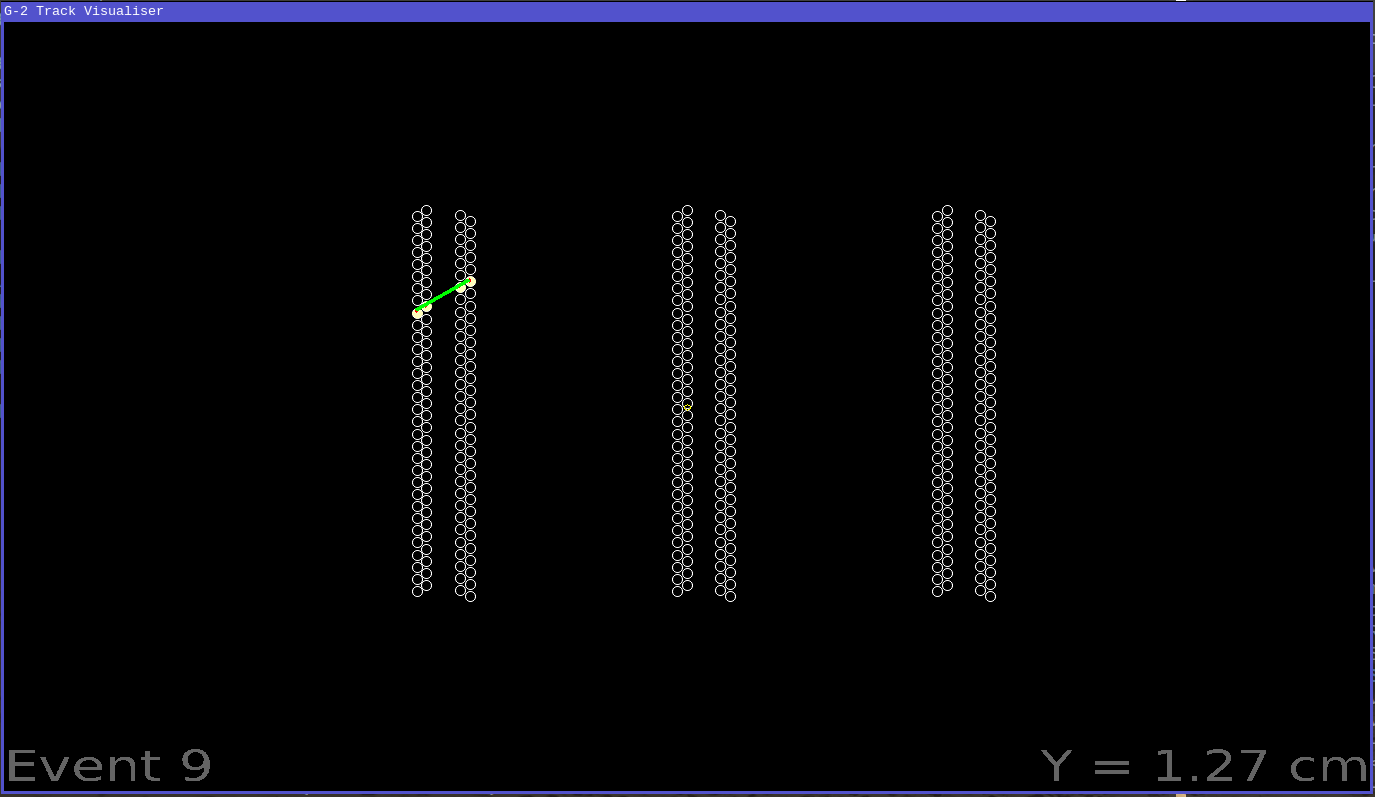
\includegraphics[width=\textwidth]{pic1}

The horizontal axis on-screen represents the 'z' axis, or along the beam pipe, while the vertical on-screen axis represents 'x', the horizontal normal to the beam. The 'y' axis of the experiment can be thought of as orthogonal to the screen, with the positive direction coming out towards the user's face. When an event is loaded by the program, it automatically displays the cross-section of the detectors at the optimal value of 'y' found by the track-finding software, and displays this value on-screen.\newline

trackervis has a relatively simple graphical and keyboard interface. Clicking and dragging translates the diagram, and the user can zoom in and out by scrolling up and down, or pressing the up and down keys. Holding \verb|alt| while scrolling will instead manually alter the value of 'y' being shown. Pressing the left and right arrows will change the event being displayed. Pressing \verb|T| will toggle the 'tally mode'. In this mode the diagram of straws will not display a single track event, but rather a kind of heat map of all the events stored in the file. Each straw is displayed as a colour corresponding to the total number of 'track event-worthy' hits that have been detected in it - the colour is stronger the greater the number of total hits in that straw.\newline

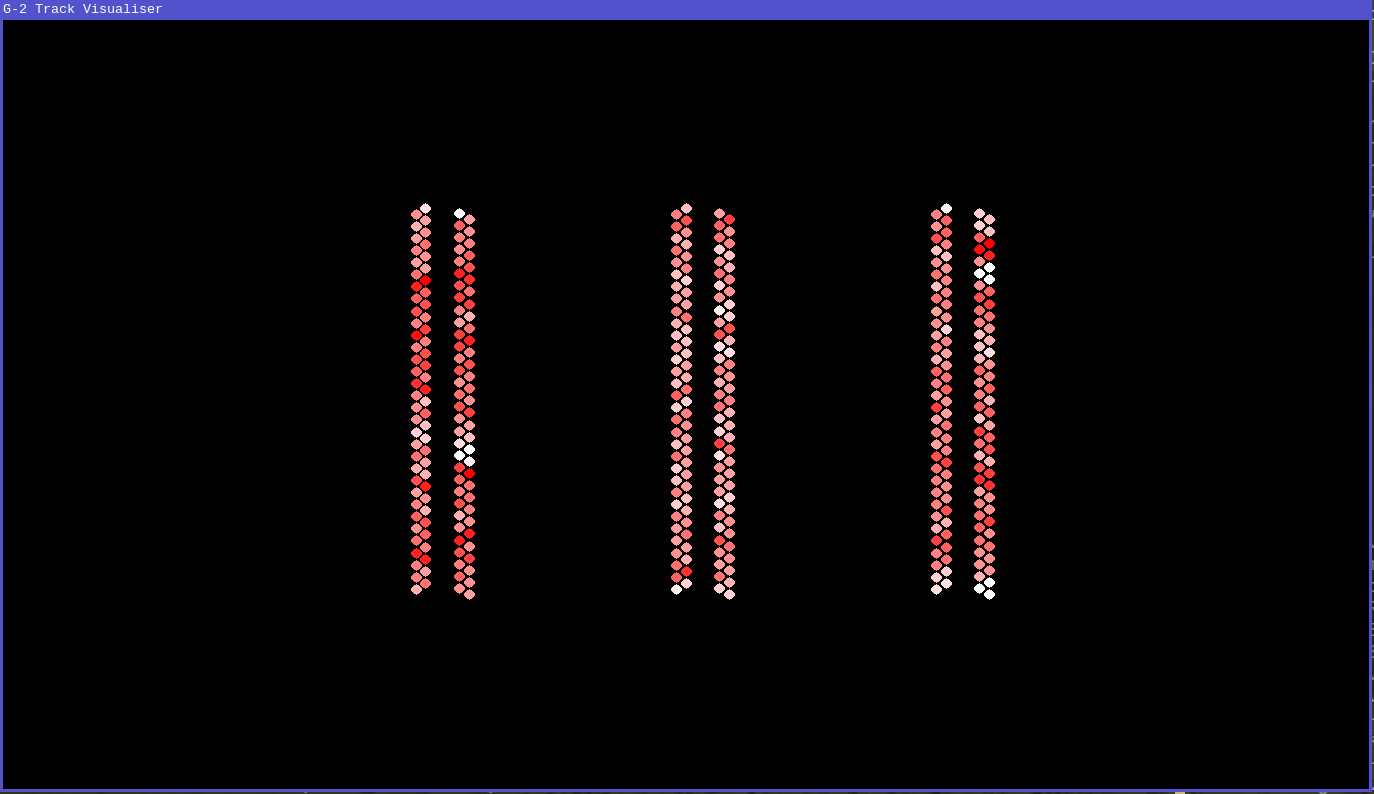
\includegraphics[width=\textwidth]{pic2}

If run without any command-line arguments, trackervis will attempt to display results from a file named 'trackevents.txt' in the same folder. If it is not found, the program will exit. To have the program use a different file, specify the file path as a command-line argument, e.g.\ \\
\verb| trackervis ../relativepath/file.txt|\ or \\
\verb| trackervis /absolutepath/file.txt|

\subsection*{Configuration File}

Trackervis comes with a limited default configuration file (with the same syntax and parsing as the track events file), which can be edited by the user, taking effect the next time the program is run. The program will check for the existence of a file named 'trackervis.conf'. If it exists, the program will parse it, and apply the custom settings if they are valid. Currently, the config file allows the option to set the program's native resolution, and whether to display the hit number and 'best Y' value.\newline

\section*{File Syntax}

The file 'trackevents.txt' is included as an example of the syntax used by the program.\newline

In general, the file must be in the libconfig format\footnote{http://www.hyperrealm.com/libconfig/libconfig.html} For trackervis specifically, the file must have the following structure:

\begin{lstlisting}[caption=Track Events Input File Example.] 
layout = {

	    modules = int
	    layers = int
	    straws = int
}

trackevents = (

	{
	module = int
	hitnum = int
	hits = (
		{
		X = float
		Z = float
		layer = int
		straw = int
		},
		...
	);
	line = {
		Z1 = float
		X1 = float
		Z2 = float
		X2 = float
		}
	Ybest = float
	},
	...
);
\end{lstlisting}

The block from lines 14-19 appears \verb|hitnum| times per \verb|hits|, where \verb|hitnum| is the number of hits belonging to that track event. The parent block (here shown from lines 10-29) appears for the total number of track events in the file.\newline
Lists are enclosed by \verb|();|. If a block of entries (enclosed in \verb|{}|) is an element of a list, all the blocks \emph{apart from the last one} must be followed by a comma (like \verb|{...},|).

\section*{Current Limitations and Potential Improvements}

Currently the program has some drawbacks:\newline

Although the number of modules/layers/straws can be specified in the \verb|layout| section of the track events file, their relative geometry is hardcoded (in the function \verb|geom_init| in \verb|vis.c|) to be that of the test data analysed by Barry King's \verb|TestStraws| program. While it might not be too difficult to alter the \verb|vis.c| source file for a given new geometry, it would perhaps be more elegant to expand the \verb|layout| section of the track events file to specify the full geometry of the system in question. It is also not currently possible to specify multiple different modules (e.g.\ different numbers of straws) in the track events file.\newline

Currently the only HEP nodes that trackervis can be installed on are the CentOS7 ones (alpha, hepcuda1), due to being the only ones with the SDL2 library installed. Programs can only be run on these (to my knowledge) from an SSH session. The limited network bandwidth to deliver the framebuffer over the SSH session appears to present a major bottleneck to the program, drastically reducing the number of frames per second experienced by the client. The program should be fast enough to run on any personal Linux computer natively, however.

\end{document}
